\paragraph{Versuchsziel}
Das Ziel des Versuches ist die Bestimmung der Lebensdauer von kosmischen Myonen.

\section{Theorie}
\label{sec:Theorie}

\subsection{Kosmische Myonen.}
Durch energiereichen Protonen, die mit den Atomen der Luftmolekülen wechselwirken, entstehen in der hohen 
Atmosphäre Pionen. Diese zerfallen wiederum wie folgt:
\begin{equation*} 
\pi^+ \to \mu^+ + \nu_{\mu} \qquad \text{ und } \qquad \pi^- \to \mu^- + \bar{\nu}_{\mu} \quad .
\end{equation*}
Die so entstandenen Myonen die sich nach dem Zerfall in Richtung Erde bewegen, tun dies mit annährend 
Lichtgeschwindigkeit. Die Myonen können mit einem Szintillationsdetektor nachgewiesen werden. 
Treffen die Myonen auf den Detektor, können sie auf dem  Weg durch die Szintillatormaterie ihre kinetische 
Energie abgegben. Dies führt dazu, dass die Szintillatormolekühle in einen angeregten Zustand übergehen und bei 
Rückkehr in den Grundzustand einen Lichtquant emittieren. Dieser kann durch einem, optisch an dem 
Szintillatormaterial gekoppelten, Sekundärelektronenvervielfachers (SEV) nachgewiesen werden. Da die Myonen auf dem
Weg zur Erde aus der hohen Atmosphäre schon einen Großteil ihrer Energie abgegebenhaben, können nun drei Fälle 
eintreten. Der erste Fall: Das Myon hat soviel Energie verloren, dass es im Szintillatiormaterial zerfällt. Dabei 
kann die Lebensdauer bestimmt werden, da sowohl beim Eintritt in den Detektor als auch beim Zerfall ein Lichtquant 
emittiert wird. Der Lichtquant der beim Zerfall entsteht ist auf das Elektron, dass beim Zerfall entsteht, 
zurückzuführen, da dieses ebenfalls das Szintillatormaterial anregt. Der zweite Fall: Es handelt sich bei dem 
Myon um ein negativ geladenes Myon und es wird vom Szintillatormaterial absorbiert. Der dritte Fall: Das 
Myon hat noch genug Energie, um sich durch das 
Szintillatormaterial und den Detektor zu bewegen. In den letzten beiden Fällen wird zwar das eintreffende Myon 
detektiert aber es kann keine Lebensdauer bestimmt werden. Die von den letzten beiden Fällen auftretenden 
Effekte müssen auch schaltungstechnisch berücksichtigt werden, dazu mehr in Kapitel \ref{sec:Aufbau}.
\subsection{Lebensdauer.}
\label{sec:Lebensdauer}
Zuerst muss die Lebensdauer $\tau$ definiert werden. Dazu wird zu erst das Zerfallsgesetz
\begin{equation} 
 N \left( t \right) = N_0 \cdot \symup{exp}\left( -\lambda t \right)
 \label{eq:ZG}
\end{equation}
betrachtet. Dabei bezeichnet $\lambda$ die Zerfallskonstante, $t$ die Zeit und $N_0$ die Gesamtanzahl der 
betrachteten Teilchen. Draus folgt dann die Expotential-Verteilung der Lebensdauern auf dem Intervall $t$ bis 
$\symup{d}t$: 
\begin{equation*}
\symup{d}N \left( t \right) = N_0 \cdot \lambda \cdot \symup{exp} \left( - \lambda t \right) \symup{d}t \; .
\end{equation*}
Den Erwartungswert dieser Verteilung zu $t$ identifizieren man mit der Lebensdauer $\tau$, daraus folgt dann: 
\begin{equation}
  <t> = \tau = \frac{1}{\lambda} \; . 
 \label{eq:tau}
\end{equation}

\subsection{Versuchsaufbau.}
\label{sec:Aufbau}
\paragraph{Grundlegende Messmethode.}
Der Aufbau ist schematisch in der Abbildung \ref{fig:aufbau} dargestellt. Der Szintillationsdetektor ist aus 
einem zylinderförmigen Edelstahltank aufgebaut, an beiden Enden ist jeweils ein SEV opitisch an das 
Szintillatormaterial gekoppelt. Der vom Szintillatormaterial abgegebene Lichtimpuls hat eine ungefähre Länge von 
\SI{10}{\nano\second}. Die Zeit ziwschen zwei Lichtpulsen, die als Folge eines Einfalls und Zerfalls eines Myon 
emittiert wurden, ist die gesuchte Messgröße. Diese kann dann mit einem Zeit-Amplituden-Konverter (TAC) 
gemessen werde. Der TAC gibt dann ein Spannungsimpuls ab, dessen Höhe proportional zum zeitlichen Abstand der 
beiden Lichtimpulse ist. Der Impuls wird dann an einen Vielkanalanalysator weitergeleitet, der das Signal 
entsprechend seiner Höhe in einem Kanal einordnet und einspeichert. Ein Rechner wird dann an den 
Vielkanalanalysator angeschlossen, dieser speichert die Daten und verarbeitet diese. Der Rechner ermittelt auch 
über nicht-linearer Ausgleichsrechnung die Lebensdauer.

\begin{figure}
  \centering
  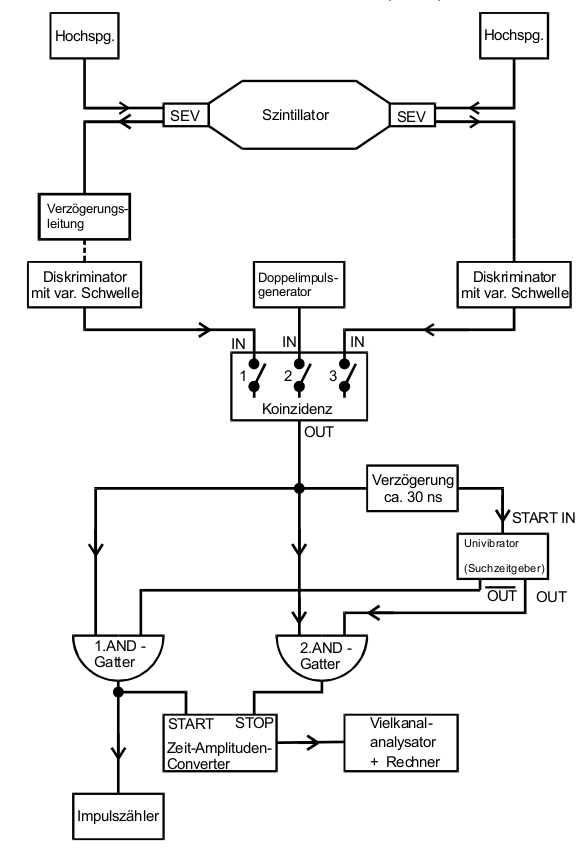
\includegraphics[height=12cm]{pics/Aufbau.png}
  \caption{Schematische Abbidung des Aufbaus aus Quelle \cite{Anleitung}.}
  \label{fig:aufbau}
\end{figure}

\paragraph{"Stop-Uhr Methode".}
Nun treten aber auch die in Kapitel 
\ref{sec:Lebensdauer} besprochenen Fälle auf, dass sich ein Myon durch den Tank bewegt ohne zu zerfallen oder mit 
dem Szintillatormaterial wechselwirkt. Folglich würde es nur einen Impuls geben und es könnte keine Lebensdauer 
bestimmt werden. Deshalb wird schaltungstechnisch verwirklicht, dass eine Messzeit $T_s$ mit einem Startimpuls 
anfängt und dann abgebrochen wird, wenn der Zerfall eingetretten ist oder nach Ablauf von $T_s$ die Messung 
abgebrochen wird und die Schaltung auf den Ausgangszustand zurückgestellt wird. In diesem Versuchsaufbau wird 
dies über eine monostabile Kippstufe (auch Univibrator genannt) und zwei AND-Gatter erreicht. An der monostabilen 
Kippstufe kann $T_s$ eingestellt werden. Am ersten AND-Gatter liegt nach einem Startimpuls ein H-Signal an. 
Nach einer Verzögerung wird die Kippstufe angestoßen. Der TAC misst nun die Zeit. Kommt es wärend der Messzeit 
$T_s$ kein Stopimpuls, der über das zweite AND-Gatter an den TAC weitergeleitet wird, dann wird die Messung 
verworfen und der TAC gibt kein Signal ab. Treffen nun zwei Myonen innerhalb $T_s$ im Tank ein, kommt es 
zu einer Fehlmessung, dies wird Untergrundrate $U$ genannt und kann über Anzahl der detektierten Myonen und der 
Messzeit $T_s$ berechnet werden. 

\paragraph{Rauschunterdrückung.}
Bei endlichen Temperaturen neigen die Photokathoden des Szintillations-Detektor zur spontaner Elektronenemission, 
das führt zu einem Spannungsimpuls obwohl kein Lichtquant eingefallen ist. Die Impulse die dabei entstehen sind 
aber klein gegen die Impulse die auftreten, wenn ein Lichtquant einfällt. Deshalb verwendet man einen 
Diskriminator, welcher alle Impulse herrausfiltert die kleiner sind als eine einstellbare Schwelle. Zudem wird 
ein zweiter SEV verwendet, da bei zu groß eingestellter Schwelle auch "echte" Impulse herrausgefilter werden. 
Der zweite SEV wird ebenfalls mit einem Diskriminator versehen und dann über eine Koinzidenzschaltung mit dem 
zweiten verbunden. Treffen zwei Impulse innerhalb einer einer Zeit $\Delta t_K$ ein, dann sendet die 
Koinzidents ein Signal aus. Folglich gibt die Koinzidents ein Impuls, wenn ein Myon von beiden SEV detektiert 
wurde, dies ist immer der Fall, zubeachten ist, dass der Lichtweg von einem SEV zum anderen SEV ca. 
\SI{4}{\nano\second} beträgt. Somit sollte $\Delta t_K$ größer als \SI{4}{\nano\second} sein. Es ist sehr 
unwahrscheinlich das beide SEV innerhalb $\Delta t_K$ jeweils ein Elektron emittieren, welches die 
Diskriminatorschwelle überschreitet. Zu beachten ist, dass aufgrund von schaltungstechnischen Unterschieden 
(z.B. Kabellängen) die Schaltungen von den SEV zur Koinzidentzschaltung aufeinander angepasst werden muss, in 
diesem Versuchsaufbau wurde dies mit einer Verzögerungsleitung verwirklicht.



